\scanpage{65}
\diagram{\begin{tikzcd}
\mathcal M\arrow[r,shift left=2pt,"\lambda_!"]\arrow[d,equal]&\mathrm{Ch}_\bullet(\mathrm{Ab})\arrow[l,shift left=2pt,"\lambda^*"]\\
M^{\unsure{\flat|h}}&
\end{tikzcd}}
$\lambda^*($

\diagram{\begin{tikzcd}[column sep=large,row sep=large]
\mathcal M\widehat\otimes\mathcal M\arrow[r,"(\lambda\boxtimes\lambda)_!"]\arrow[d,"\delta_M^*"']&\mathrm{Ch}_{\bullet\bullet}(\mathrm{Ab})\arrow[d,"\int=\delta_{\mathrm{ch}_\bullet}^*"]\\
\mathcal M\arrow[r,"\lambda_!"']&\mathrm{Ch}_\bullet(\mathcal M)
\end{tikzcd}}
\figure{\begin{tikzpicture}\draw[->](0,0) to[bend left=25](1.1,1);\end{tikzpicture}}
\diagram{\begin{tikzcd}
\mathrm{ch}_\bullet(\mathrm{Ab})^{\unsure{\flat|h}}\simeq\mathrm{Ch}_\bullet(\mathrm{Ab})&\mathrm{Ch}_{\bullet\bullet}^{\unsure{a}}(\mathrm{Ab})\arrow[l]
\end{tikzcd}}
\diagram{\begin{tikzcd}
\deleted{\unsure{C}}\ \mathrm{ch}_\bullet(\mathrm{Ab})\arrow[r]&\mathrm{ch}_{\bullet\bullet}(\mathrm{Ab})\quad??
\end{tikzcd}}
\figure{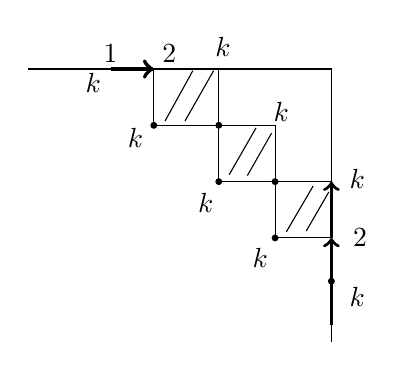
\begin{tikzpicture}[scale=1.1]
\draw(-1.2,2.7)--(2.3,2.7)--(2.3,-.45);
\draw[line width=1.5pt,->](-.25,2.7)--(.25,2.7);
\draw(.25,2.7)--(.25,2.05)--(1,2.05)--(1,1.4)--(1.65,1.4)--(1.65,.75)--(2.3,.75);
\draw(1,2.7)--(1,2.05)--(1.65,2.05)--(1.65,1.4)--(2.3,1.4);
\draw[line width=1.2pt,->](2.3,-.25)--(2.3,.75);
\draw[line width=1.2pt,->](2.3,.75)--(2.3,1.4);
\foreach \x/\y in {.25/2.05,1/2.05,1/1.4,1.65/1.4,1.65/.75,2.3/.25}{\fill(\x,\y)circle(.04);}
\draw(.38,2.1)--(.7,2.68);\draw(.61,2.1)--(.94,2.68);
\draw(1.12,1.48)--(1.43,2.02);\draw(1.33,1.47)--(1.61,1.96);
\draw(1.78,.82)--(2.09,1.35);\draw(2.01,.83)--(2.27,1.28);
\node at(-.25,2.88){$1$};\node at(.43,2.88){$2$};\node at(1.05,2.96){$k$};
\node at(-.45,2.54){$k$};\node at(.04,1.9){$k$};\node at(1.72,2.2){$k$};
\node at(.85,1.16){$k$};\node at(2.6,1.43){$k$};\node at(1.48,.52){$k$};
\node at(2.63,.75){$2$};\node at(2.6,.07){$k$};
\end{tikzpicture}}
\figure{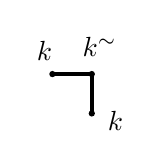
\begin{tikzpicture}[line width=1.3pt]
\draw(0,.5)--(.5,.5)--(.5,0);\fill(0,.5)circle(.04);\fill(.5,.5)circle(.04);\fill(.5,0)circle(.04);
\node at(-.1,.8){$k$};\node at(.6,.85){$k^\sim$};\node at(.8,-.1){$k$};
\end{tikzpicture}}
\diagram{\begin{tikzcd}[column sep=small]
L_{\unsure{i+1}}\arrow[r,dash]&L_i\arrow[r,dash]&L_{i-1}\\
\mathbin{\text{---}}k\arrow[r,dash]\arrow[u]&k\arrow[r,dash]\arrow[u]&0
\end{tikzcd}}
\deleted{$\operatorname{Hom}($}
\[
\operatorname{Hom}(\underbrace{L_\bullet}_{\in\mathrm{ch}_\bullet(\mathrm{Ab})},\int M_{\bullet\bullet})
\simeq\operatorname{Hom}(\underbrace{\delta(L_\bullet)}_{\in\mathrm{ch}_{\bullet\bullet}(\mathrm{Ab})\,?},M_{\bullet\bullet})
\]
\figure{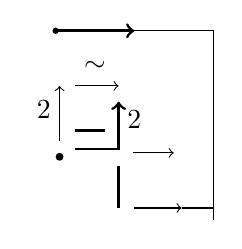
\begin{tikzpicture}
\draw[->,line width=1pt](0,1.9)--(1,1.9);\draw(1,1.9)--(2,1.9)--(2,-.5);
\fill(0,1.9)circle(.04);\fill(.05,.3)circle(.05);
\draw[->](.05,.5)--(.05,1.2);\node at(-.15,.9){$2$};
\draw[->](.25,1.2)--(.8,1.2);\node at(.5,1.45){$\sim$};
\draw[->,line width=1pt](.25,.4)--(.8,.4)--(.8,1);\node at(1,.77){$2$};
\draw[line width=1.2pt](.25,.63)--(.63,.63);\draw[->](.98,.35)--(1.5,.35);
\draw[line width=1pt](.8,.18)--(.8,-.35);\draw[->](1,-.35)--(1.6,-.35);\draw(1.6,-.35)--(2,-.35);
\end{tikzpicture}}
\[
L_\bullet=a
\]
\deleted{$\unsure{\delta L_\bullet}$}
\deleted{$\operatorname{Hom}(a,M_{0,0})=$}
\deleted{$M_{0,1}\unsure{+}M_{1,0}$}

\diagram{\begin{tikzcd}
\lambda_!(a\otimes y)\arrow[r,"\deleted{\unsure{asph}}\inserted{\text{qu.iso}}"]&\lambda_!(a)\otimes\lambda_!(y)
\end{tikzcd}}
\diagram{\begin{tikzcd}
\lambda^*(\xi\otimes\eta)&\lambda^*(\xi)\otimes\arrow[l,"\unsure{\sim}"]
\end{tikzcd}}
\diagram{\begin{tikzcd}[column sep=large]
\lambda^*(L_\bullet\otimes M_\bullet)\arrow[r,leftrightarrow,"\substack{W_M\ ?\\\deleted{\text{qu.iso}}}"]&\lambda^*(L_\bullet)\otimes\lambda^*(M)
\end{tikzcd}}
\diagram{\begin{tikzcd}
M\otimes M\arrow[r,"\lambda\boxtimes\lambda"]&\mathrm{Ch}_{\bullet\bullet}(\mathrm{Ab})\\
M\arrow[u,"\delta_M"]\arrow[r,"\lambda"']&\mathrm{Ch}_\bullet(\mathrm{Ab})\arrow[u,"\delta"']
\end{tikzcd}}
\diagram{\begin{tikzcd}[column sep=large,row sep=large]
L_\bullet\otimes M_\bullet\quad\deleted{\unsure{M\otimes}}&
\lambda_!(\lambda^*(L_\bullet)\otimes\lambda^*(M))\arrow[l,"\text{qu.iso ?}"']\arrow[d,"\text{qu.iso}\quad\mathbf{EZ}"]\\
&\lambda_!(\lambda^*(L_\bullet))\otimes\lambda_!(\lambda^*(M))\arrow[ul]
\end{tikzcd}}
\[
M\otimes\mathbf M
\]
$\lambda^*$
\diagram{\begin{tikzcd}
P=M\otimes M\\M\arrow[u]
\end{tikzcd}}
$\operatorname{Hom}(x\boxtimes y,z)$
\diagram{\begin{tikzcd}(M\otimes M)^{\unsure{\flat|h}}\arrow[d]&\\M^{\unsure{\flat|h}}&\end{tikzcd}}
\diagram{\begin{tikzcd}\mathbf M\arrow[r]&P\end{tikzcd}}
\diagram{\begin{tikzcd}
M^{\unsure{\flat|h}}\arrow[r,shift left=2pt,"i_!"]\arrow[r,dash,shift right=7pt,"i_*"']&P^{\unsure{\flat|h}}\arrow[l,"\unsure{i^*}"]
\end{tikzcd}}
\mspage{64}
